% ----------------------------------------------------------------
% Descrição do Trabalho, relevância e abordagens.
% ----------------------------------------------------------------
\chapter{Introdução}
\label{introducao}
%\addcontentsline{toc}{chapter}{Introdução}

\section{Contexto}

As metodologias de previsão espacial dividem a área de estudo em pequenas subáreas, que podem ter tamanhos e formas distintas, ou podem ser subáreas homogêneas e de lados iguais (quadrículas) e quadradas. As quadrículas são usadas para formar uma grade, ou um mapa de quadrículas, que  apresenta vantagens em relação às outras formas de divisão, pela possibilidade de se aumentar a resolução, dependendo apenas da entrada de dados.

Tal  divisão em mapa de quadrículas (grade) tem sido aplicada em diversos métodos de previsão espacial de carga \cite{willis2002spatial}, \cite{melo2012multi}, \cite{arango2004spatial}. Assim é possível obter uma representação gráfica, em forma de uma imagem, da distribuição de densidade de cargas, de modo a determinar um crescimento, seja de carga ou de qualquer outra forma de densidade em um ponto da grade, que seja esperado para aquela pequena área. 

Para se fazer o planejamento espacial de áreas urbanas é necessário a criação de uma metodologia que forneça informações bem definidas para o planejamento de expansão destas regiões urbanas, tendo em vista que toda informação regional possa ser usada para definir melhores localizações e minimizar os custos de implantação de sistemas e equipamentos.Por exemplo, no caso de densidade de carga, os sistemas elétricos de distribuição podem ter ser remanejados ou instalados em regiões urbanas de forma a minimizar os custos destes tipos de atividades \cite{willis2007spatial}.    

Alguns métodos de previsão espacial executam simulações \cite{arango2004spatial}, \cite{carreno2011cellular} de crescimento partindo de dados diferenciados no tempo, de modo que o crescimento de cada quadrícula não dependa de outros valores, resultando assim, em metodologias capazes de identificar curvas de crescimento para regiões seguindo heurísticas que usam apenas destes dados diferenciados. 

Outras técnicas de previsão de regiões urbanas consideram a taxa de crescimento das pequenas regiões (quadrícula) como sendo a mesma da taxa de habitantes naquela regão, provindos de mapas de uso da terra \cite{wu2002data}. Outras variações ainda trazem métodos que avaliam a chance de uma região crescer, fazendo cálculos probabilísticos \cite{melo2015spatial}, \cite{arango2004spatial} para definir se uma determinada região irá ou não se desenvolver.

Geralmente as técnicas de previsão espacial são aplicadas à densidade de carga, e englobamos dados de toda uma área urbana\cite{willis2007spatial}, de modo que algumas regiões, mais externas ou distantes são ignoradas para não gerar ruído na previsão. Porém, todas as regiões de uma determinada área devem ser consideradas por terem a capacidade de influenciar no crescimento de carga das áreas mais centrais \cite{willis2002spatial}.

As quadrículas são regiões quadradas e que devem representar o mundo real em posição, sendo que se pode atribuir mais valores àquela região, como densidade de carga. O tamanho da quadrícula define se uma grade de quadrículas (ou mapa de quadrículas) estará em alta resolução ou em baixa resolução. SEDAC o Centro de Dados e Aplicações Socioeconômicas, é um dos Centros de Arquivos Ativos Distribuídos (DAACs) no Sistema de Dados e Informação do Sistema de Observação da Terra (EOSDIS) da Administração Nacional de Aeronáutica e Espaço dos Estados Unidos (NASA). Com foco nas interações humanas no meio ambiente, o SEDAC tem a missão de desenvolver e operar aplicações que suportem a integração de dados socioeconômicos e de ciências da terra e serve como um "Portal de Informação" entre ciências da terra e ciências sociais. 

Neste centro de dados apresentam-se diversos mapas em quadrículas em baixa resolução (por exemplo, o mapa de densidade populacional \emph{GPWv4: Population Density - 2015} \cite{SEDAC2016} como pode ser visto na figura \ref{fig:sedacGPWv4}) sobre diversos tópicos, tendo suas quadrículas com o área aproximada de 1 \(milha^2\). Em baixa resolução é possível identificar grosseiramente grandes regiões de crescimento, porém vários detalhes são deixados de lado. Neste trabalho busca-se um refinamento na previsão, usando quadrículas de áreas muito menores, porém existem alguns problemas em se usar uma alta resolução nos estudos de previsão, relacionados \cite{longley1996spatial}, como a demanda por uma alta quantidade de informações para a caracterização da grade, grande esforço computacional no processamento dos dados, que geralmente dependo do número da entrada de dados e da técnica de previsão usada. Porém, permite a criação em alta resolução do mapa de quadrículas, melhorando a visualização, análise e diversos outros fatores para a previsão. 

\begin{figure}[h]
	\centering	
	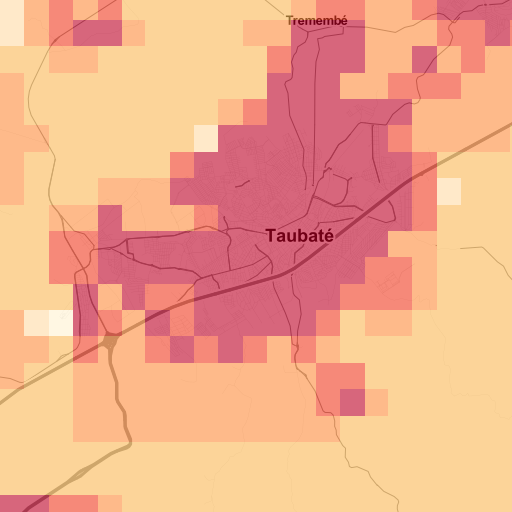
\includegraphics[scale=1]{Figuras/sedacGPWv4.png}
	\caption{\emph{GPWv4: Population Density - 2015} com foco na cidade de Taubaté }
	\label{fig:sedacGPWv4}
\end{figure}

O método de efetuar uma previsão espacial de alta resolução deve considerar como entrada diversos fatores \cite{willis2002spatial}, requer uma grande quantidade de dados, e neste caso, leva em consideração o crescimento local através da obtenção de características regionais usando matrizes de convolução e fatores de ponderação para se obter o crescimento de cada pequena região (quadrícula) de modo que não se ignore nenhuma região e também que tais regiões não ignoradas não venham a causar erros na previsão das demais regiões. Assim, divide-se o mapa de quadrículas em sub regiões compostas por quadriculas, de modo que a previsão ocorra naquela região independente das demais, evitando assim, que regiões mais distantes prejudiquem o processamento de previsão das demais regiões.

A previsão espacial de carga de cada região é feita através do uso de uma função de previsão que tem como entrada, um mapa base \cite{willis2002spatial} e valores otimizados pelo algoritmo competitivo imperialista \cite{atashpaz2007imperialist} modificado \cite{roche2011imperialist} e otimizado (com alterações propostas neste artigo), que por sua vez possui uma função semelhante à função de previsão, porém que possui rotinas para buscar quais valores são os ideais a serem usados para previsão de períodos à frente do mapa base.

São construídos diversos mapas da mesma região, durante diversos períodos diferentes, espaçados igualmente no tempo, para que se possa ser feita uma previsão espacial como uma série temporal de mapas de quadrículas. Algoritmos evolutivos já vem sendo usados para calcular parâmetros de entrada para funções de previsão de séries temporais \cite{whitehead1996cooperative}. No caso de \citeauthor{whitehead1996cooperative}, é criado um algoritmo genético (GA) \cite{mitchell1998introduction} cooperativo-competitivo capaz de evoluir os centros e larguras de uma rede neural RBF \cite{ren2006rbfnn} para ser aplicado na previsão de uma série temporal. Neste trabalho portanto, usa-se o algoritmo competitivo imperialista (ICA) para evoluir valores de uma função proposta capaz de fazer uma "regressão", usando fatores de ponderação e matrizes de convolução para a previsão de crescimento densidade espacial em mapas bidimensionais.

Em resumo, apresenta-se uma técnica capaz de fazer previsão espacial de densidades, sejam elas de quaisquer tipo (carga, populacional, etc.), em alta resolução, que considera diversos fatores na construção dos mapas de quadrículas e que ainda não deixa de ignorar nenhuma área mais afastada da região central urbana, podendo assim melhorar inferência dos resultados obtidos dos métodos de previsão espacial de baseados em quadrículas. 

\section{Objetivos}

O objetivo deste trabalho é efetuar a previsão de densidade espacial genérica (qualquer que seja o parâmetro analisado, densidade de carga, densidade populacional, etc.) sobre um período curto de tempo (de 6 meses a 5 anos), com capacidade de previsão sobre dados dispostos em alta resolução.

Para isto, desenvolve-se uma metodologia capaz de traduzir um conjunto de dados para um histórico de mapas de uma localização que então serão processados por um algoritmo evolutivo, que irá gerar indivíduos capazes de gerar previsões de 1 ou mais períodos a frente com vantagem sobre os modelos estatísticos convencionais. 

Mais especificamente, este trabalho aborda os seguintes tópicos:
\begin{itemize}
\item Modelagem e normalização dos dados para utilização dentro da aplicação.
\item Transformação dos dados iniciais em mapas da mesma localização, durante diferentes períodos, de acordo com o foco da previsão.
\item Regionalização dos mapas para previsão.
\item Definição de uma função de avaliação capaz de fazer previsão espacial sobre regiões.
\item Aplicação do processo evolutivo para definir a melhor curva de crescimento para cada pequena área de uma região.
\item Utilização do resultado do processamento evolutivo para criar as previsões desejadas.
\item Analisar as diferenças entre as previsões geradas pelo modelo proposto com o valores reais e comparar com o modelo de previsão convencional. 
\end{itemize}

\section{Revisão Bibliográfica}
Nesta seção são apresentados, trabalhos que possam servir como base para o desenvolvimento, trabalhos que possuam alguma relação com o objetivo, além de terem suas ideias discutidas para a solução do problema proposto em questão. Alguns conceitos simples e essenciais para o desenvolvimento da metodologia ou experimentos também podem vir a ser abordados.

Um dos conceitos básicos para se iniciar o desenvolvimento de uma metodologia de previsão espacial é a forma com que se definirá o espaço de trabalho e como os dados serão modelados para que o objetivo seja atingido. A proposta deste trabalho é trazer uma metodologia capaz de resultar em uma previsão de espacial sobre áreas urbanas. Assim, é necessário que se utilize dados que traduzam a realidade para os dados a serem processados, convertendo-os e ajustando-os de modo preciso para que não existam erros durante a aquisição e tradução dos dados reais.

Neste caso, este trabalho explora a filosofia de quadrículas, que diz respeito ao particionamento de uma região em pequenas regiões, para a previsão espacial de cargas aplicadas nestas pequenas áreas. Este modelo é apresentado por \citeauthor{willis2002spatial} \cite{willis2002spatial} que enfatizam que o planejamento de sistemas de potência deve sempre incluir a previsão de distribuição de carga, pois tais planos de expansão são baseados em diversas proposições, relacionadas ao crescimento futuro da carga, mesmo que este venha ser definido inadequadamente, seja forçado ou implícito. Assim, ao se utilizar este modelo, consegue-se aumentar a precisão da previsão para atender as necessidades do planejamento. No caso deste trabalho fazemos uma generalização da filosofia para que o modelo possa representar quaisquer tipos de dados, sejam eles do setor elétrico ou qualquer outro.

Atualmente, este método, conhecido também como previsão de pequenas áreas (\emph{small area forecast}) \cite{willis1995spatial}, é amplamente usado para previsão espacial do crescimento do consumo de carga. Não existe um critério fixo para a separação da região em pequenas regiões, porém, a mais comumente utilizada é a separação em regiões não uniformes, tais que cada uma represente uma região correspondente ao mapeamento elétrico da área de distribuição, sendo esta divisão definida por critérios como área de distribuição de subestações, ou áreas de atuação de concessionárias etc.. Outra forma, é a separação em regiões uniformes, quadradas que se encaixam em diversas situações, por manter o toda região homogênea e normalizada, denominada a filosofia de quadrículas ou quadriculamento da região. A Figura \ref{fig:RegionsAndQuadrics} mostra como pode ser dividido um mapa de uma região usando ambos os modelos citados no parágrafo anterior. 

\begin{figure}[h]
	\centering	
	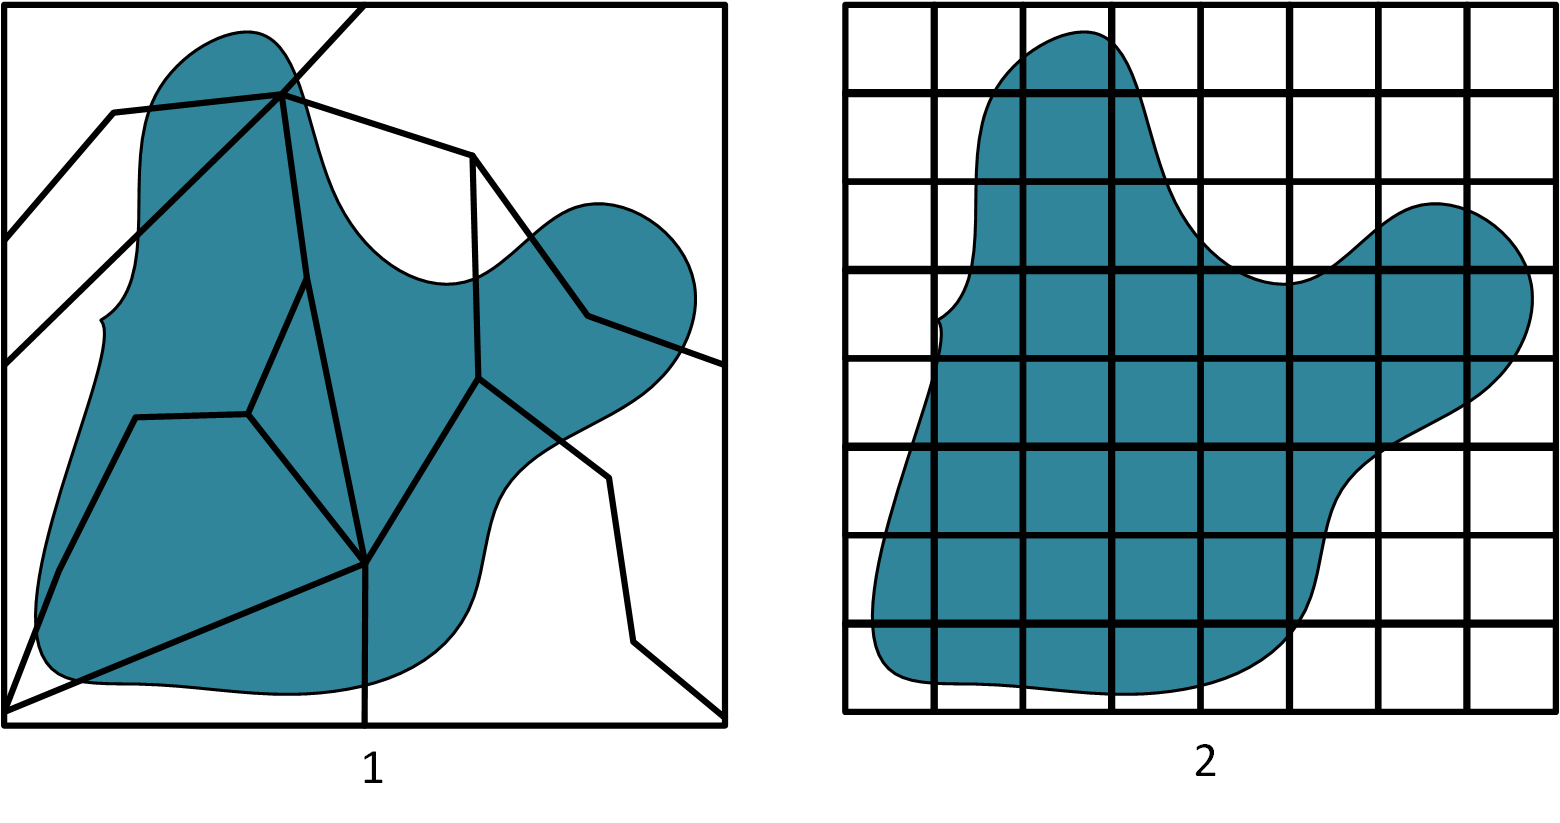
\includegraphics[scale=0.55]{Figuras/RegionsAndQuadrics.png}
	\caption{Regiões e Quadrículas}
	\label{fig:RegionsAndQuadrics}
\end{figure}

Ambas possuem vantagens e desvantagens segundo \citeauthor{willis2002spatial} \cite{willis2002spatial}, como por exemplo, a separação por quadrículas, ilustrada no item 2 da figura, pode produzir melhores resultados, porém pode ser mais complexo obter e processar os dados para formar as regiões. E a separação por regiões apesar de possuir sua separação formada por dados que classificam a região de alguma forma, é mais complexa de ser modelada computacionalmente para análise homogênea, pois suas área são de tamanhos e formas diferentes.

Existem muitos métodos de previsão de pequenas áreas, portanto eles sempre se encaixam em uma das duas categorias (definido por \citeauthor{willis2002spatial} \cite{willis2002spatial} e detalhado por \citeauthor{arango2000thesis} \cite{arango2000thesis}, sendo:

\begin{itemize}
\item Métodos de ajuste, que considera a curva de tendência do crescimento de períodos passados, ajustando-a através de métodos como mínimos quadrados, média móvel, etc. de modo que os períodos futuros possam ser extrapolados a partir desta curva ajustada.
\item Métodos baseados no uso da terra, que faz as previsões futuras baseando-se na análise de fatores de uso da terra, como planos diretores, zoneamentos, entre outros, os quais possam ser retiradas informações de como os crescimentos de carga (de regiões residenciais, industriais ou comerciais) irão crescer durante os períodos futuros.
\end{itemize}

No caso deste trabalho, o método desenvolvido se aplica principalmente ao primeiro modelo de métodos, apesar de processar os dados obtidos de modo que eles sejam transformados em informações de crescimento de carga residencial durante os períodos, ao processar tais dados, leva-se em consideração como estes dados crescem ao longo dos períodos, de modo que se possa gerar uma curva de tendência e extrapolar uma previsão de períodos futuros. O segundo método é usado apenas inicialmente, ao se ajustar os dados para que eles possam ser normalizado e traduzidos para um mapa de quadrículas, porém não se faz nenhum tipo de previsão ou geração de regras de previsão durante esta etapa de tradução.

Um modelo dinâmico de expansão de cargas é proposto por \citeauthor{arango2000thesis}, e baseia-se em conceitos de análise locacional, que aplica a teoria dos polos urbanos e se encaixa mais nos métodos baseados no uso da terra (segundo item). Deste modo, ele cria um simulador de expansão de cargas que evolui de forma dinâmica e continua as condições para uma nova unidade de carga. Tal modelo consegue representar a expansão de carga, usando uma adaptação do processo de recozimento simulado que fora especificamente desenvolvido para solucionar o problema. Este trabalho traz uma solução mais genérica, para a previsão de expansão de densidades, seja ela de cargas, populacional, entre outras.

Uma análise interessante sobre o erro de previsão espacial é desenvolvida por \citeauthor{arango2000thesis}, que avalia o erro de previsão espacial considerando as diferenças entre os valores reais e estimados para cada subárea urbana, e traz um exemplo muito bom, que demonstra a preocupação para com a avaliação da imprecisão dos modelos de previsão espacial. No exemplo ele imagina duas regiões, as quais tenham uma magnitude total de cargas iguais, porém distribuídas diferentemente, como mostra a Figura \ref{fig:ErrorDistArango}.

\begin{figure}[h]
	\centering	
	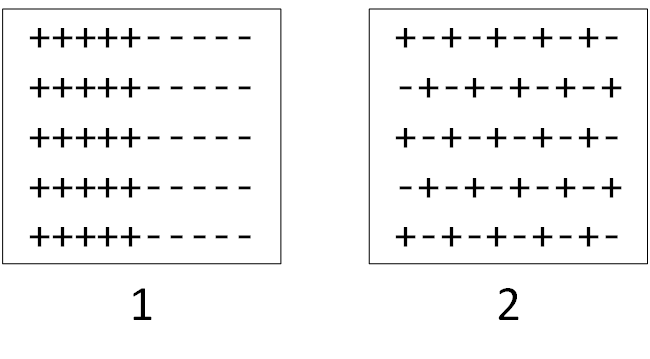
\includegraphics[scale=2]{Figuras/Ilustration-ErrorDistArango.png}
	\caption{Distribuições distintas do mesmo erro global, detalhado em \cite{arango2000thesis} e definido por \cite{willis1995spatial}}
	\label{fig:ErrorDistArango}
\end{figure}

A estimativa para ambas as áreas serão completamente distintas, sendo que na primeira existe uma tendencia bem direcionada e na segunda ocorrerá uma estimativa muito mais homogênea em relação a região. 

Ao se fazer uma análise estatística entre a uma região estimada e sua região real, comparando o erro absoluto de cada pequena área (quadrícula). É possível ocorrer que uma região seja estimada de forma absolutamente correta, assim como também pode ocorrer que uma região seja estimada de forma totalmente incorreta. Neste trabalho trabalha-se para que tais erros sejam minimizados de modo a fazer com que toda região tenha uma estimativa com o menor erro possível, seguindo as taxas de crescimento tanto das pequenas áreas, quanto da região como um todo, e ainda, também agrega o crescimento das pequenas áreas presentes nas redondezas da pequena área que esteja sendo analisada.

Para o desenvolvimento da aplicação foi necessária inicialmente a modelagem dos dados iniciais de modo que estes fossem convertidos com a menor ou nenhuma quantidade de erro residual. Pois neste caso, os dados estão representados em coordenadas geográficas, e são utilizadas diversos cálculos de distância para que eles sejam adequadamente identificados em sua pequena região. Para se calcular a distância entre dois pontos, dispostos em um mapa terrestre em coordenadas cartesianas, pode-se aplicar o teorema de Pitágoras:

\[d = \sqrt{(X2 - X1)^2 + (Y2 - Y1)^2}\]

Sendo \((X1, X2)\) e \((Y1,Y2)\) os pontos iniciais e finais de longitude e latitude respectivamente.

Esta fórmula de cálculo de distância, quando aplicada a pontos cuja distância é menor que 20 km, produz erros dependentes de suas posições reais dispostas no globo, sendo que tais erros variam como:
\begin{itemize}
\item De 0 a 30 metros para latitudes menores que 70 graus.
\item De 0 a 20 metros para latitudes menores que 50 graus. 
\item De 0 a 9 metros para latitudes menores que 30 graus.
\end{itemize}

Tal gestão de erros é desnecessária quando se usa a distância calculada pela fórmula de Haversine \cite{shumaker1984astronomical}, que calcula a distância entre dois pontos dispostos na superfície de uma esfera, relacionando os lados aos ângulos de uma esfera triangular. Assim, fazendo o uso de um mapa terrestre esférico, onde tal esfera possui raio \(R\), e tendo a representação dos pontos que se deseja calcular a distância como vetores compostos na forma (Longitude, Latitude), temos que o \(ponto1 = (lon1,lat1)\) e o \(ponto2 = (lon2,lat2)\), calculamos a distância como mostra a expressão:

\[dlon = lon2 - lon1\]
\[dlat = lat2 - lat1\]
\[a = \sin^2\left(\frac{dlat}{2}\right) + \cos(lat1) \cdot \cos(lat2) \cdot \sin^2\left(\frac{dlon}{2}\right)\]
\[c = 2 \cdot \arcsin(\min(1,\sqrt{a}))\]
\[d = R \cdot c\]

A distância calculada resulta em um valor exato, tanto computacionalmente quanto matematicamente, onde \(c\) é a distância do caminho mais curto entre os dois pontos, denominada ortodromia, representada em radianos, que multiplica \(R\), convertendo o resultado de d para a mesma unidade do Raio \(R\). 

A função \(min\) protege contra possíveis erros de arredondamento que podem sabotar a computação do arco-seno caso os dois pontos estejam em lados opostos da terra. Sob estas condições, a Fórmula Haversine é mal condicionada, mas o erro, que talvez pareça grande, que chega a ser de aproximadamente 2 km, está no contexto de uma distância próxima 20,000 km, sendo que este erro é de aproximadamente 0.00001\% da distância total.

No ambiente computacional, a maioria das funções ou componentes trigonométricos são expressados em radianos. Uma vez que os dados de coordenadas (Longitude e Latitude) geralmente estão expressos na forma Graus, Minutos e Segundos, é necessário convertê-los para graus decimais:

\[
\begin{matrix}
coordDec = 
& coordGMS.Graus +\\ 
& \left(\frac{CoordGMS.Minutos}{60}\right) +\\ 
& \left(\frac{CoordGMS.Segundos}{3600}\right)
\end{matrix}
\]

Com as coordenadas convertidas para graus decimais, ainda é necessário convertê-las para radianos, que é simplesmente multiplicar a coordenada em graus decimais por \(\frac{\pi}{180}\):

\[coordRad = \frac{coordDec \cdot \pi}{180}\]

Por fim, a definição de \(R\) como sendo o raio da esfera, deve ser levado em consideração que o planeta Terra não é uma esfera perfeita, mas sim, possui uma forma chamada esferóide oblato (Figura \ref{fig:OblateSpheroid}), e portanto, deve-se considerar diferentes raios para diferentes posições de latitude, uma vez que o achatamento ocorre nos polos.  

\begin{figure}[h]
	\centering	
	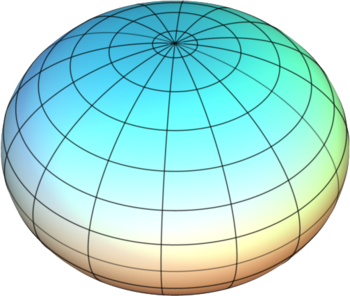
\includegraphics[scale=0.3]{Figuras/OblateSpheroid.PNG}
	\caption{Esferóide oblato}
	\label{fig:OblateSpheroid}
\end{figure}

A circunferência oficial terrestre é de 40003.2 km, que provém da definição de uma milha náutica, que historicamente é definida como 1 arco de minuto medido, à superfície média do mar, ao longo de um qualquer grande círculo da Terra. Como a terra não é uma esfera, tal definição é ambígua. Então, o valor aceito internacionalmente(SI) para uma milha náutica é de exatamente 1.852 km. Deste modo, define-se como circunferência terrestre, o valor de 40003.2 km:

\[40003.2 (km) = 360(grau) * 60\left(\frac{minuto}{grau}\right) * 1.852\left(\frac{km}{minuto}\right)  \]

Implicando então que o raio \(R\) seja de:

\[R = \frac{40003.2}{(2 \cdot \pi)} = 6367 (km) \]

Como o planeta Terra não é representado por uma esfera, mas sim por um esferóide oblato, e possui um Raio Polar de 6357 km e um raio equatorial de 6378 km, uma aproximação satisfatória seria como mostra a expressão:

\[R = 6378 - 21 \cdot \sin(lat) \]

Porém, tal aproximação é dependente apenas do valor de latitude, e o raio da curvatura é dependente não só do valor de latitude, mas também da direção, de acordo com \cite{snyder1987map}. Então, usa-se:

\[R = \frac{ a \cdot (1 - e^2)}{ (1 - e^2 \cdot \sin^2(lat))^\frac{3}{2}}\]

Onde \(a\) é o raio equatorial, \(b\) o raio polar, e \(e\) é a excentricidade do 
\(\text{elipsóide} = \left(1 - \frac{b^2}{a^2}\right)^\frac{1}{2}\). 
Então tem-se que \(e = 0.0167086\). Assim, haverá um erro mínimo sempre que as distâncias entre dois pontos de coordenadas geográficas forem calculadas utilizando a fórmula de haversine.

Este trabalho utiliza-se muito da fórmula de haversine para converter os dados iniciais, dispostos em coordenadas geográficas, para coordenadas cartesianas, de modo que se crie uma matriz de pequenas áreas (quadrículas), onde estas pequenas áreas possam vir a ser usadas para gerar um mapa cartesiano que represente fielmente os dados que foram convertidos, tanto para o processamento destes dados quanto para a apresentação dos resultados.

A previsão espacial apresentada por este trabalho é efetuada usando-se um algoritmo que classifica-se como evolutivo, isto é, está na mesma categoria que algoritmos como algoritmos genéticos (AG) \cite{mitchell1998introduction} e otimização por enxame de partículas (PSO). \cite{atashpaz2007imperialist} apresenta o algoritmo imperialista competitivo (ICA), que atinge resultados tão bem quanto algoritmos genéticos, atingindo o mínimo global geralmente ao mesmo tempo que o algoritmo genético. 

A vantagem do ICA sobre o GA se dá em relação média do custo de toda população, onde o GA geralmente fica estagnado em um patamar devido ao fato de que sempre que ocorrem mutações, seleções ou criação de novos indivíduos para complementar a população, estes indivíduos são gerados com valores aleatórios, impossibilitando a convergência de toda a população para a solução ótima. O ICA por sua vez consegue fazer com que toda a população seja convergida para a solução ótima, sem que fique estagnado ou ceia em mínimos locais.  

Outra sutil vantagem que o ICA possui sobre o GA é o fato de seus atributos serem valores numéricos de ponto flutuante, uma vez que no GA em sua versão canônica, utilizam-se vetores de atributos binários, que, desta forma, seria sempre necessário traduzir o valor do cromossomo para valores numéricos. 

Este trabalho utiliza um grande conjunto de números de ponto flutuante para sua função de avaliação, que são traduzidos para estruturas usadas pela função. Caso o vetor de atributos fosse de valores binários, seriam necessária uma tradução dos valores binários para valores numéricos de ponto flutuante, antes mesmo de se gerar as estruturas usadas pela função de avaliação, tornando este processo muito mais complexo.

\cite{roche2011imperialist} traz uma aplicação concreta do ICA voltado para otimizar o uso de ferramentas que definem estrategicamente a alocação de unidades de geração de energia para as usinas de acordo com diversos parâmetros. O ICA é comparado com modelos convencionais, como AG e PSO, tendo uma efetividade maior tanto em previsão quanto em velocidade. Voltando o Foco para a o desenvolvimento do ICA feito por \citeauthor{roche2011imperialist}, ele desenvolveu o ICA na linguagem Java, que pode ser acessado pelo repositório git em github.com/robinroche/jica \cite{jica}, sendo desenvolvido em uma linguagem orientada a objetos, de forma simples. Este trabalho propõe uma melhora na implementação orientada a objetos para o ICA de modo que ele possa ser usado genericamente para qualquer caso ou aplicação, de modo que a modelagem de qualquer problema seja rápida, prática, modular e sem a necessidade de alterar o código fonte principal da lógica do ICA. 

Tendo conhecimento que o desenvolvimento de uma metodologia para previsão espacial apresenta uma solução de alta complexidade, exige elevada quantidade de informação e a qual se deve levar em conta diversos fatores de crescimentos aleatórios e/ou imprevisíveis (como desejo político ou planejamento externo), tais problemas apresentam soluções de domínio não lineares. Assim, este trabalho propõe uma implementação diferenciada do ICA de forma que este seja capaz de atender a todas as requisições do problema de forma prática, precisa e rápida. 

A metodologia empregada faz uso do ICA para previsão espacial, em um ambiente (neste caso, urbano) bidimensional (2D). Então, para que tal problema possa ser solucionado de modo que múltiplas alterações sejam executadas e testadas afim de se obter os melhores resultados, algumas adaptações foram imprescindíveis ao ICA tanto em relação a otimização de seu desempenho na busca de soluções melhores em um tempo menor  quanto a organização e modelagem do conceito, que se deu na forma de uma implementação orientada a objetos \cite{booch1982object} e \cite{coad1991object}. 

A primeira preocupação durante o desenvolvimento foi encontrar quais seriam as abordagens mais certeiras e inovadoras para que a previsão de densidade espacial urbana fornecesse resultados aceitáveis. Tendo isto em mente, sabia-se que deveriam ocorrer diversos testes com diversas funções de avaliação diferentes, e ainda, que tais funções, devido a complexidade do problema, também teriam de ser diversas vezes ajustadas durante os testes. Assim, a aplicação dos conceitos de orientação a objetos foram utilizados para a modelagem do ambiente, para a implementação dos conceitos do ICA e de diversas funções de avaliação ou modelos de problemas diferentes.





\section{Estrutura da Dissertação}


Este documento está dividido nos capítulos: Introdução, Metodologia, Desenvolvimento, Experimentos e Resultados e Conclusão.

No capítulo introdução é contextualizado o conceito de previsão espacial urbana, que pode ser feita a partir de diversos métodos e técnicas. Também são apresentados os objetivos definidos e a justificativa da realização do trabalho.

Em Metodologia são detalhados os principais conceitos e técnicas pesquisados e aplicados no trabalho, abrangendo principalmente o Algoritmo Imperialista Competitivo e a operação matemática de convolução.

O capítulo Desenvolvimento descreve especificamente como as técnicas escolhidas foram desenvolvidas, modificadas e implementadas focando nos objetivos e na solução do problema.

Já no capítulo Experimentos e Resultados são apresentados como o ambiente foi modelado, como o método proposto se comportou sobre uma e sobre muitas regiões, e apresentação dos resultados sobre dados reais, apresentando os resultados em forma de imagens de alta resolução e uma tabela comparativa.

Por fim, no capítulo Conclusão são considerados os resultados obtidos frente aos objetivos propostos, a colaboração deste trabalho, assim como a indicação de trabalhos futuros para a continuidade da pesquisa.



